\chapter{Planejamento}
O risco pode ser compreendido matematicamente como o produto da probabilidade de ocorr�ncia de um risco e o impacto. J�, cat�strofe � o impacto somado com logaritmo neperiano da probabilidade de ocorr�ncia do risco.

\section{Fun��o para otimiza��o}

\subsection{Risco}
A fun��o Risco � definida tal que
\begin{equation}
	f(P,i) = Pi
	\label{eq:funcao_risco}
\end{equation}
onde $P \in \left[ 0; 1 \right]$ indica a probabilidade de ocorr�ncia de um risco e $i$ indica o impacto esperado quando o risco ocorrer. A Figura \ref{fig:risco} apresenta o formato da fun��o quando $i = 20$
\begin{figure}[H]
	\begin{center}
		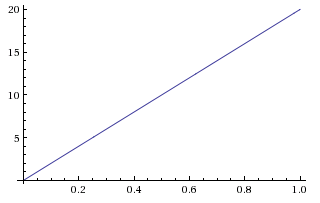
\includegraphics[width=0.5\textwidth]{img/risco.png}
		\caption{Fun��o Risco para i = 20.}
		\label{fig:risco}
	\end{center}
\end{figure}

\subsection{Cat�strofe}
A fun��o Cat�strofe � definida tal que
\begin{equation}
	g(P,i) = i + \ln (P)
	\label{eq:funcao_catastrofe}
\end{equation}
onde $P \in \left[ 0; 1 \right]$ indica a probabilidade de ocorr�ncia de um risco e $i$ indica o impacto esperado quando o risco ocorrer. A Figura \ref{fig:catastrofe} apresenta o formato da fun��o quando $i = 20$
\begin{figure}[H]
	\begin{center}
		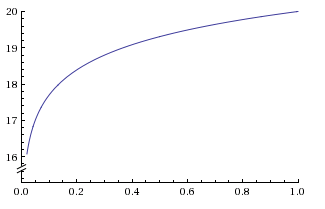
\includegraphics[width=0.5\textwidth]{img/catastrofe.png}
		\caption{Fun��o Cat�strofe para i = 20.}
		\label{fig:catastrofe}
	\end{center}
\end{figure}

Sobrepondo as duas fun��es, o objetivo � encontrar o \textit{pareto front} ou o conjunto de solu��es dominantes para as duas fun��es acima, levando em considera��o que existe um custo m�ximo a ser satisfeito. A Figura \ref{fig:funcoes_otimizacao} apresenta as fun��es \ref{eq:funcao_risco} e \ref{eq:funcao_catastrofe} sobrepostas.

\begin{figure}[H]
	\begin{center}
		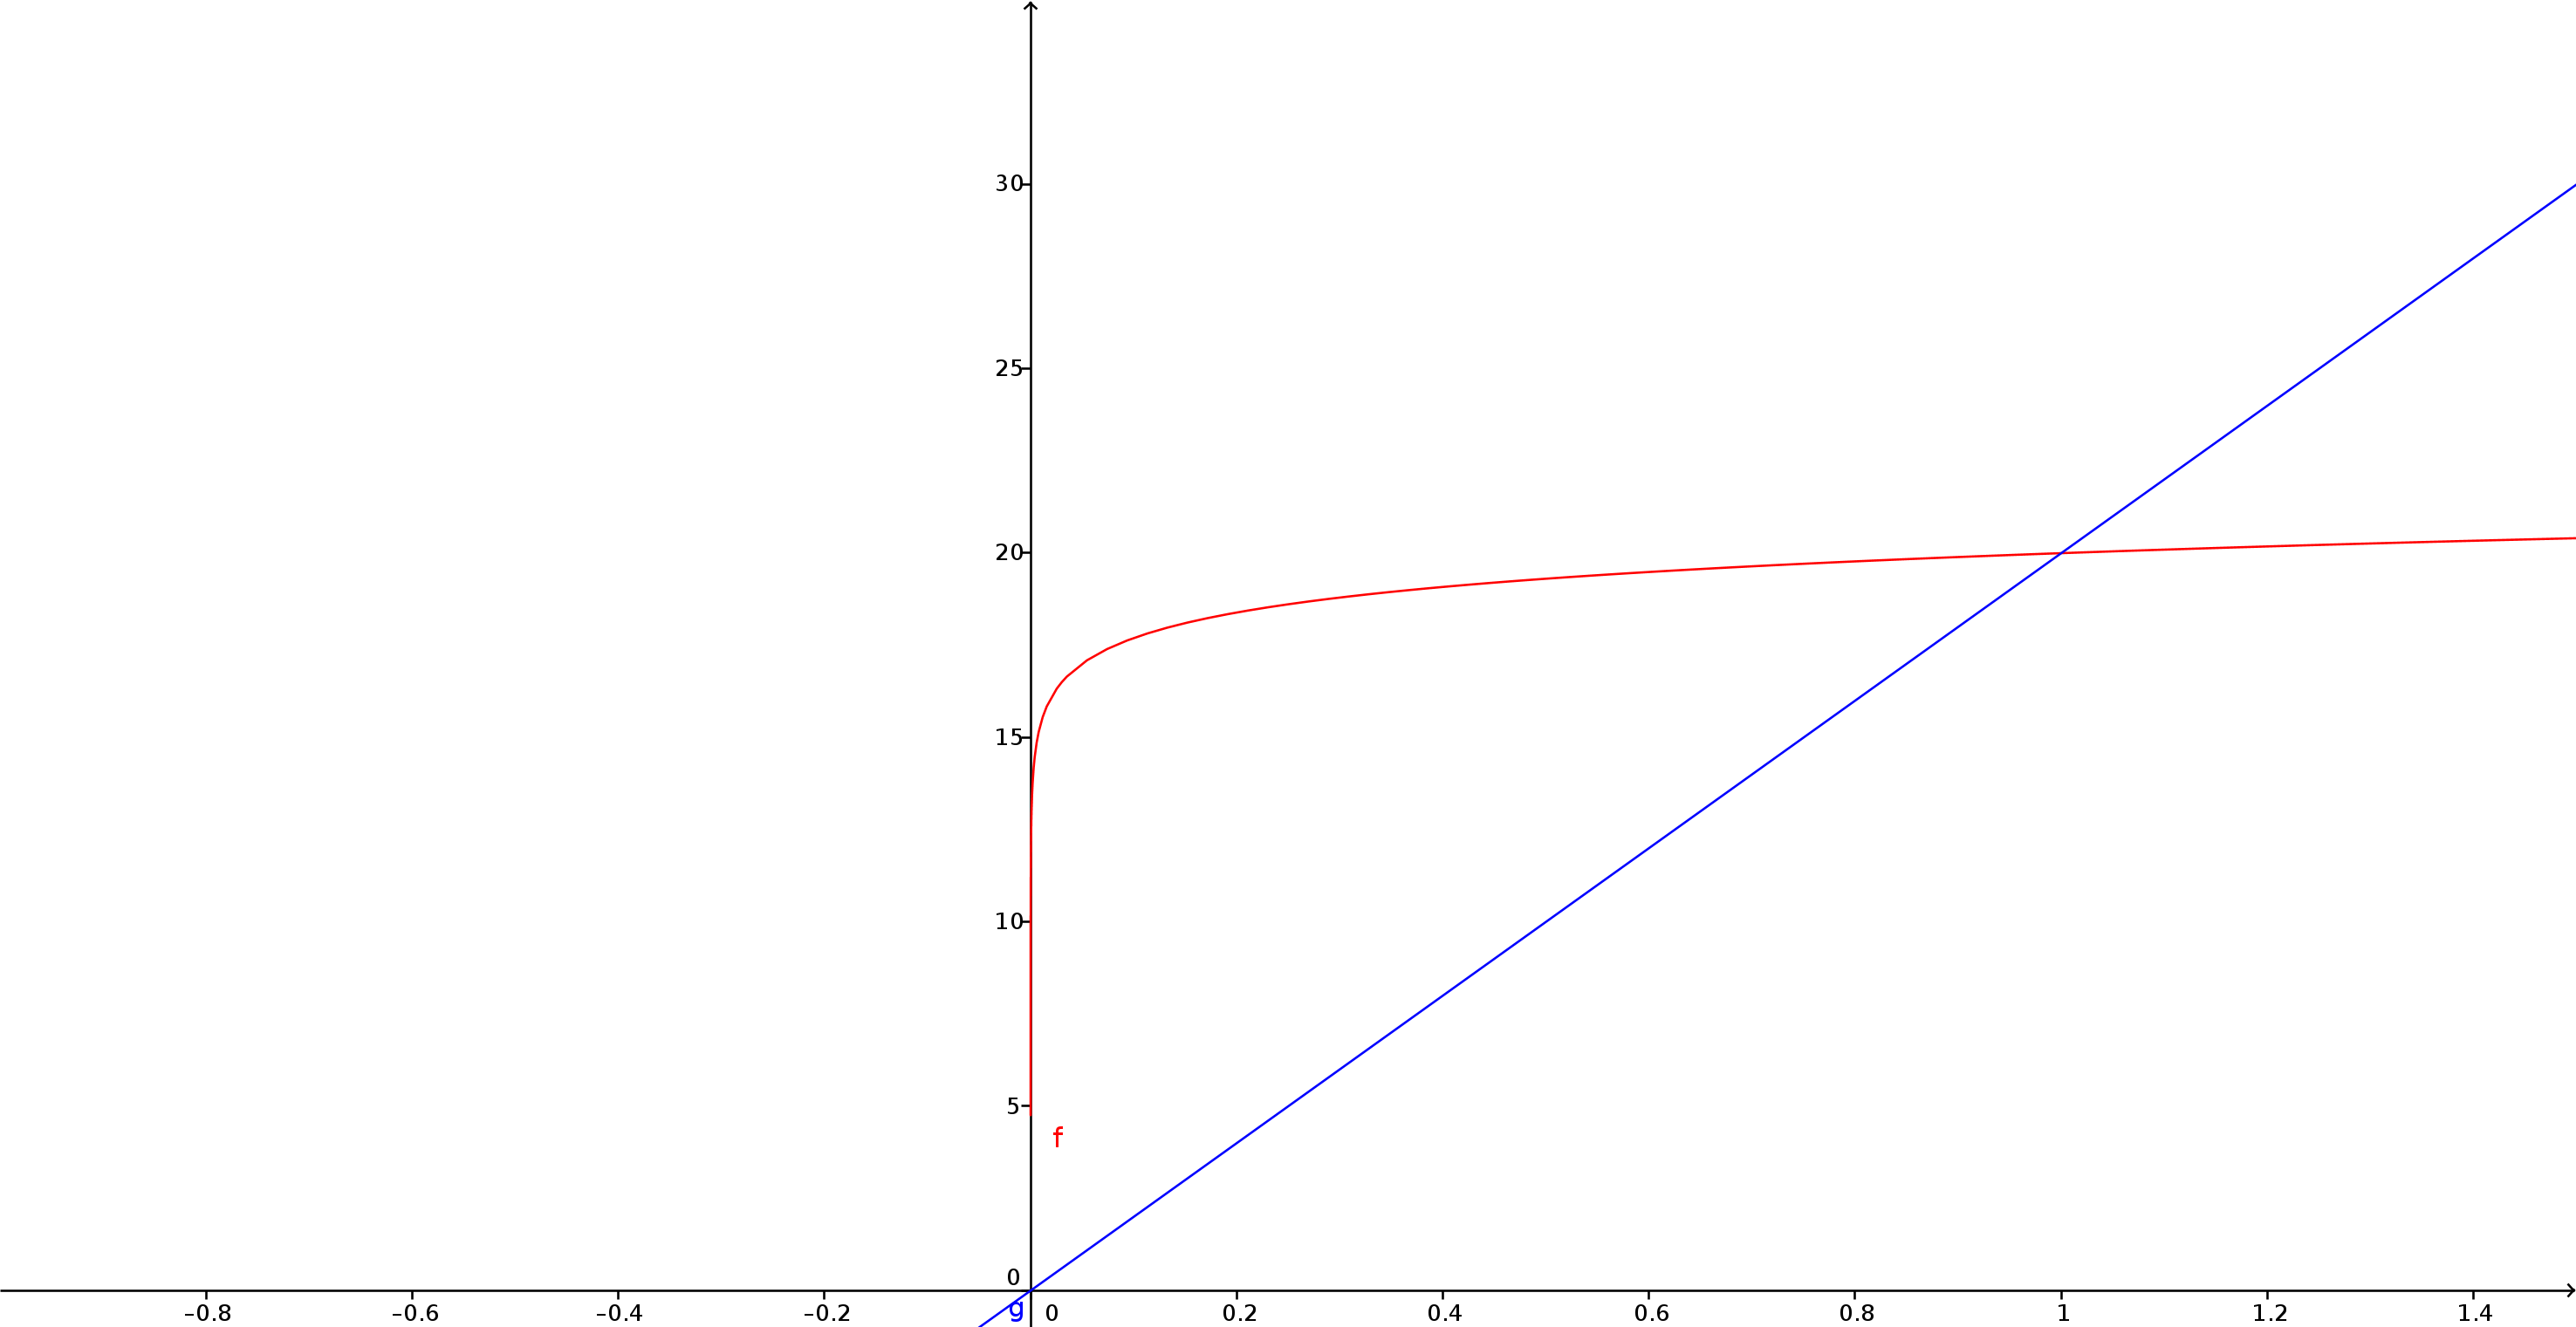
\includegraphics[width=0.8\textwidth]{img/funcoes_otimizacao.png}
		\caption{Fun��es Risco e Cat�strofe Sobrepostas para i = 20.}
		\label{fig:funcoes_otimizacao}
	\end{center}
\end{figure}